\subsection{Sprostitev definicijskega območja histogramov} \label{podpoglavje-4-1}

Če hočemo, da imata poljubna histograma enake meje stolpcev, moramo najprej uskladiti definicijski območji histogramov.

Naj bo $X$ urejen seznam z mejami stolpcev prvega histograma in $Y$ urejen seznam z mejami stolpcev drugega histograma. Za spodnjo mejo:
\begin{itemize}
	\item Če je $\min(X) > \min(Y)$, potem na začetek seznama $X$ vstavimo element $\min(Y)$. Tako v prvem histogramu dobimo še en stolpec z mejami $\min(Y)$ in $\min(X)$. Dodelimo mu vrednost $0$.
	\item Če je $\min(X) < \min(Y)$, potem na začetek seznama $Y$ vstavimo element $\min(X)$. Tako v drugemu histogramu dobimo še en stolpec z mejami $\min(Y)$ in $\min(X)$. Dodelimo mu vrednost $0$.
\end{itemize}
Za zgornjo mejo:
\begin{itemize}
	\item Če je $\max(X) < \max(Y)$, potem na konec seznama $X$ vstavimo element $\max(Y)$. Tako v prvem histogramu dobimo še en stolpec z mejami $\max(X)$ in $\max(Y)$. Dodelimo mu vrednost $0$.
	\item Če je $\max(X) > \max(Y)$, potem na konec seznama $Y$ vstavimo element $\max(X)$. Tako v drugem histogramu dobimo še en stolpec z mejami $\max(Y)$ in $\max(X)$. Dodelimo mu vrednost $0$.
\end{itemize}
Dobili smo torej največ dva nova stolpca. Ker smo jima dodelili vrednost $0$, ploščina histograma ostaja enaka, torej je bil to dober korak k našemu cilju (da bodo ploščine histogramov čim bližje 1). Definicijsko območje obeh histogramov je na sedaj enako.

\begin{zgled}

Poglejmo si primer, kako sprostimo definicijsko območje histograma.

\begin{figure}[!bh]
    \centering
    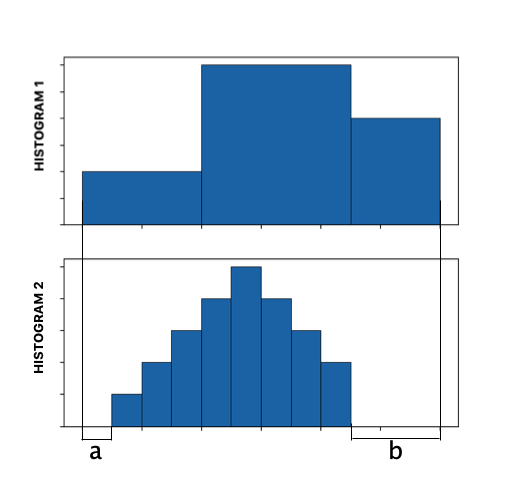
\includegraphics[scale=0.7]{definicijskoobmocje}
    \caption{Sprostitev definicijskega območjahistograma 2. Dobili smo dva nova stolpca ain b.}
\end{figure}

\end{zgled}